 	\documentclass[aspectratio=169]{beamer}

\usepackage[utf8]{inputenc}

\usepackage{graphicx}
\usepackage{caption}
\usepackage{subfigure}

\graphicspath{{pictures/}}
\DeclareGraphicsExtensions{.pdf,.png,.jpg}

\usepackage{amsmath,amsfonts,amssymb,amsthm,mathtools}
\usepackage[main=russian,english]{babel}
%\usepackage[T1]{fontenc}

\title{Фильтр Лио}
\date{\small{МФТИ, Долгопрудный 2022}}
\author{\small{Крейнина Матвея \\ студент 2 курса группы Б05-005}}


\usetheme{texsx}
%\usetheme{gcr2019}

\begin{document}
%1	-	Титульный слайд
\begin{frame}
  \frametitle{\textcolor{white}{Вопрос по выбору}} 
	\titlepage
\end{frame}

%3	- Фильтр Вуда
\begin{frame}
\frametitle{\textcolor{white}{Фильтр Вуда}}


\begin{figure}[h]
\begin{minipage}[h]{0.49\linewidth}
Этот прибор состоит из пластинки одноосного кристалла C, вырезанной параллельно оптической оси, помещенной между двумя поляризаторами A и B. Оси поляризаторов устанавливаются параллельно, а ось кристаллической пластинки составляет с ними угол 45\textdegree.
\end{minipage}
\begin{minipage}[h]{0.49\linewidth}
\center{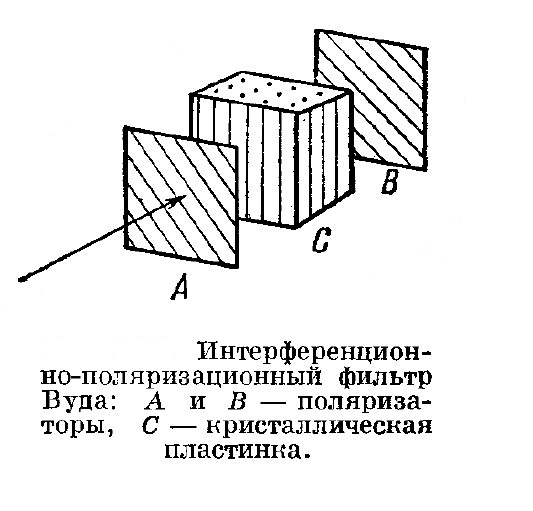
\includegraphics[scale = 0.45]{01.jpg}}
\end{minipage}
\end{figure}

\end{frame}

%4 -- Продолжение фильтра Вуда
\begin{frame}
\frametitle{\textcolor{white}{Разность хода}}

Поляризованный пучок света в пластинке C расщепляется на два одинаково направленных, равных по интенсивности и поляризованных во взаимно перпендикулярных направлениях пучка света. Эти пучки света будут распространяться в кристалле с разными скоростями $v_0 = \frac{c}{n_0}$ и $v_e = \frac{c}{n_e}$, где $n_0$ и $n_e$ -- показатели преломления для обыкновенного и необыкновенного лучей. 



Разность их хода будет равна: $\Delta = d \cdot (n_e - n_0)$. Когда разность хода равна целому числу длин волн, мы получаем плоско поляризованный свет с первоначальной ориентацией плоскости поляризации.
    


\begin{center}
    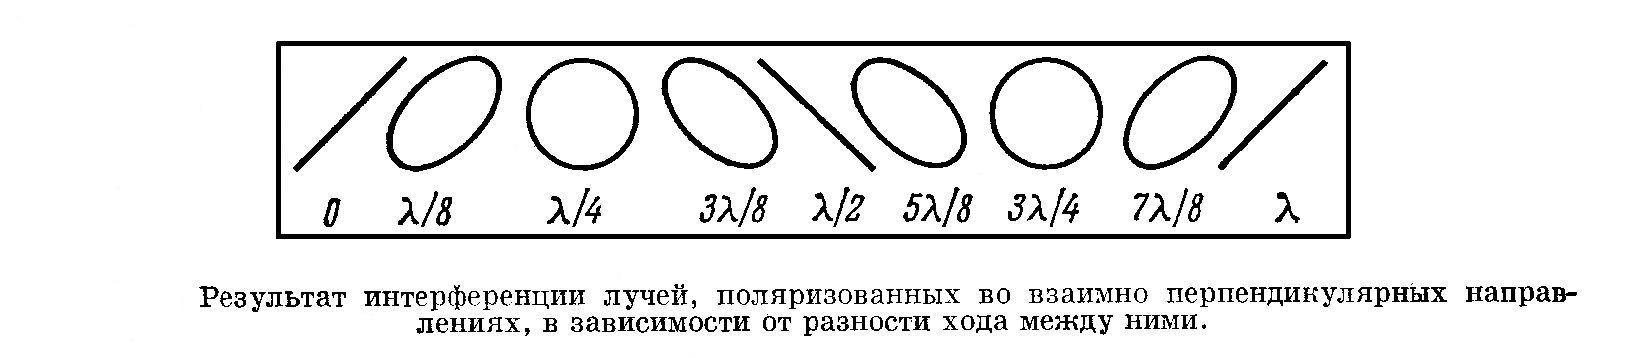
\includegraphics[scale=0.4]{02.jpg}
\end{center}
\end{frame}

%Задача по теме...
\begin{frame}
\frametitle{\textcolor{white}{Вывод формулы}}
\begin{figure}[h]
\begin{minipage}[h]{0.59\linewidth}
Рассмотрим следующую задачу: есть $N + 1$ поляроидов и $N$ пластинок кварца, главные направления всех поляроидов параллельны и составляют угол 45 \textdegree с оптической осью пластинок. Волна поляризована вдоль главного направления поляроида, а толщины пластинок равны $d, 2d, ..., 2^{N-1}d$. Показатели преломления кварца $n_e, n_0$, амплитуда на входе равна $A_0$.

\end{minipage}
\begin{minipage}[h]{0.39\linewidth}
\center{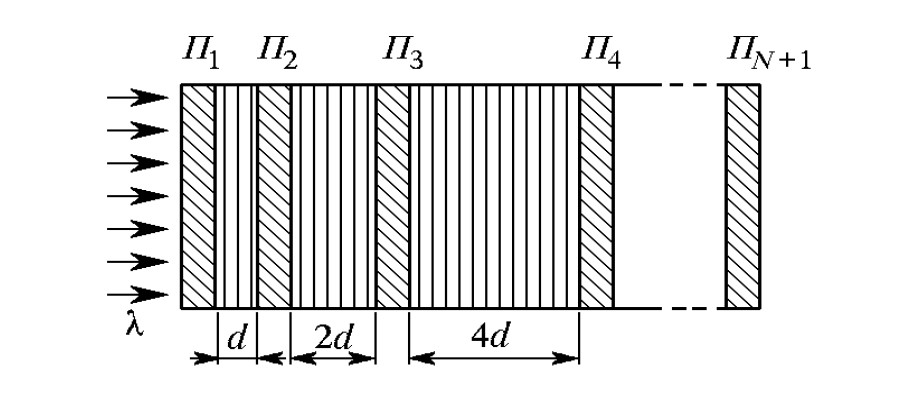
\includegraphics[scale = 0.33]{05.jpg}}
\end{minipage}
\end{figure}

Найдем амплитуду волну на выходе и коэффициент пропускания.
\end{frame}

\begin{frame}
\frametitle{\textcolor{white}{Решение}}
После первой пластинки у нас будет две волны с амплитудами $A_0 /\sqrt2$ и ортогональными поляризациями. После второй их амплитуды уменьшатся до $A_0 / 2$. Сдвиг фаз будет равен: $\phi = kd(n_0 - n_e)$. Каждая из этих волн пройдя, вторую пластинку и третий поляроид разделится каждая на две волны с амплитудами $A_0 / 4$ и взаимными фазами $0, \phi, 2\phi, 3\phi$. После поляроида с номером $N+1$ будет сумма волн, которую мы подсчитаем следующим образом:

\begin{equation*}
    E = \frac{A_0}{2^N} \sum\limits_{m = 0}^N \exp^{i m \phi} = \frac{A_0}{2^N} \frac{1 - \exp^{i 2^N \phi}}{1 - \exp^{i \phi}}
\end{equation*}

Амплитуда на выходе будет равна: 
\begin{equation*}
    A = |E| = \frac{A_0}{2^N} \frac{\sin \left( 2^N \phi / 2 \right)}{\sin \left(\phi / 2 \right)}
\end{equation*}

\end{frame}

%5 -- Формулы для Вуда
\begin{frame}
\frametitle{\textcolor{white}{Пропускание}}
Коэффициент пропускания:
\begin{equation*}
T = \cos^2 \left( \pi \frac{(n_e - n_0)d}{\lambda} \right)
\end{equation*}


Он не учитывает потери на отражение и поглощение света элементами, из которых состоит фильтр, и потерь в первом поляризаторе, которые составят 50 \% для естественного света. Последние равны нулю для плоско поляризованного света с соответствующей ориентацией плоскости поляризации.



Коэффициент пропускания имеет ряд максимумов ($T = 1$) и минимумов ($T = 0$) для следующих длин волн:
\begin{equation*}
    \lambda_{max} = \frac{1}{k} (n_e - n_0) d \quad
    \lambda_{min} = \frac{2}{2k + 1}(n_e - n_0) d
\end{equation*}

\end{frame}

\begin{frame}
\frametitle{\textcolor{white}{Применение фильтра Вуда}}

Поэтому такой фильтр может служить лишь для гашения отдельных спектральных линий и пропускания других. Обычно его используют для выделения одной из двух близко расположенных линий.

Спектральный интервал между соседними максимумом и минимумом пропускания фильтра, определяющий полуширину полосы пропускания, легко найти, как:
\begin{equation*}
    \Delta \lambda = \lambda_{max} - \lambda_{min} = \frac{\lambda_{max}}{2k +1} = \frac{\lambda^2}{2 (n_e - n_0) d}
\end{equation*}

Расстояние между максимумами соотвественно в два раза больше.

Можем оценить толщину фильтра, которая необходима для подавления одной из двух близкий линий, разделленных интервалом $\Delta \lambda$.

Фильтр для подавления одной из компонент резонансного дублета натрия (5889.95; 5895.92 \AA), который сделан из кварцевой пластинки $(n_e - n_0) = 0.00911$. Такой фильтр будет иметь толщину 32 мм. Такой же фильтр, но из кальцита $n_e-n_0 = 0.1719$ имеет толщину примерно в 18.9 раз меньшую, т.е. 1.7 мм.
\end{frame}

%6 Фильтр Вуда
\begin{frame}
\frametitle{\textcolor{white}{Фильтр Лио}}
Бернадр Лио предложил монохроматический фильтр, состоящий из стопы фильтров Вуда с толщинами пластинок, увеличивающимися в геометрической прогрессии с показателем 2. При этом выходной поляризатор первого фильтра служит входным поляризатором второго и т.д.

\begin{center}
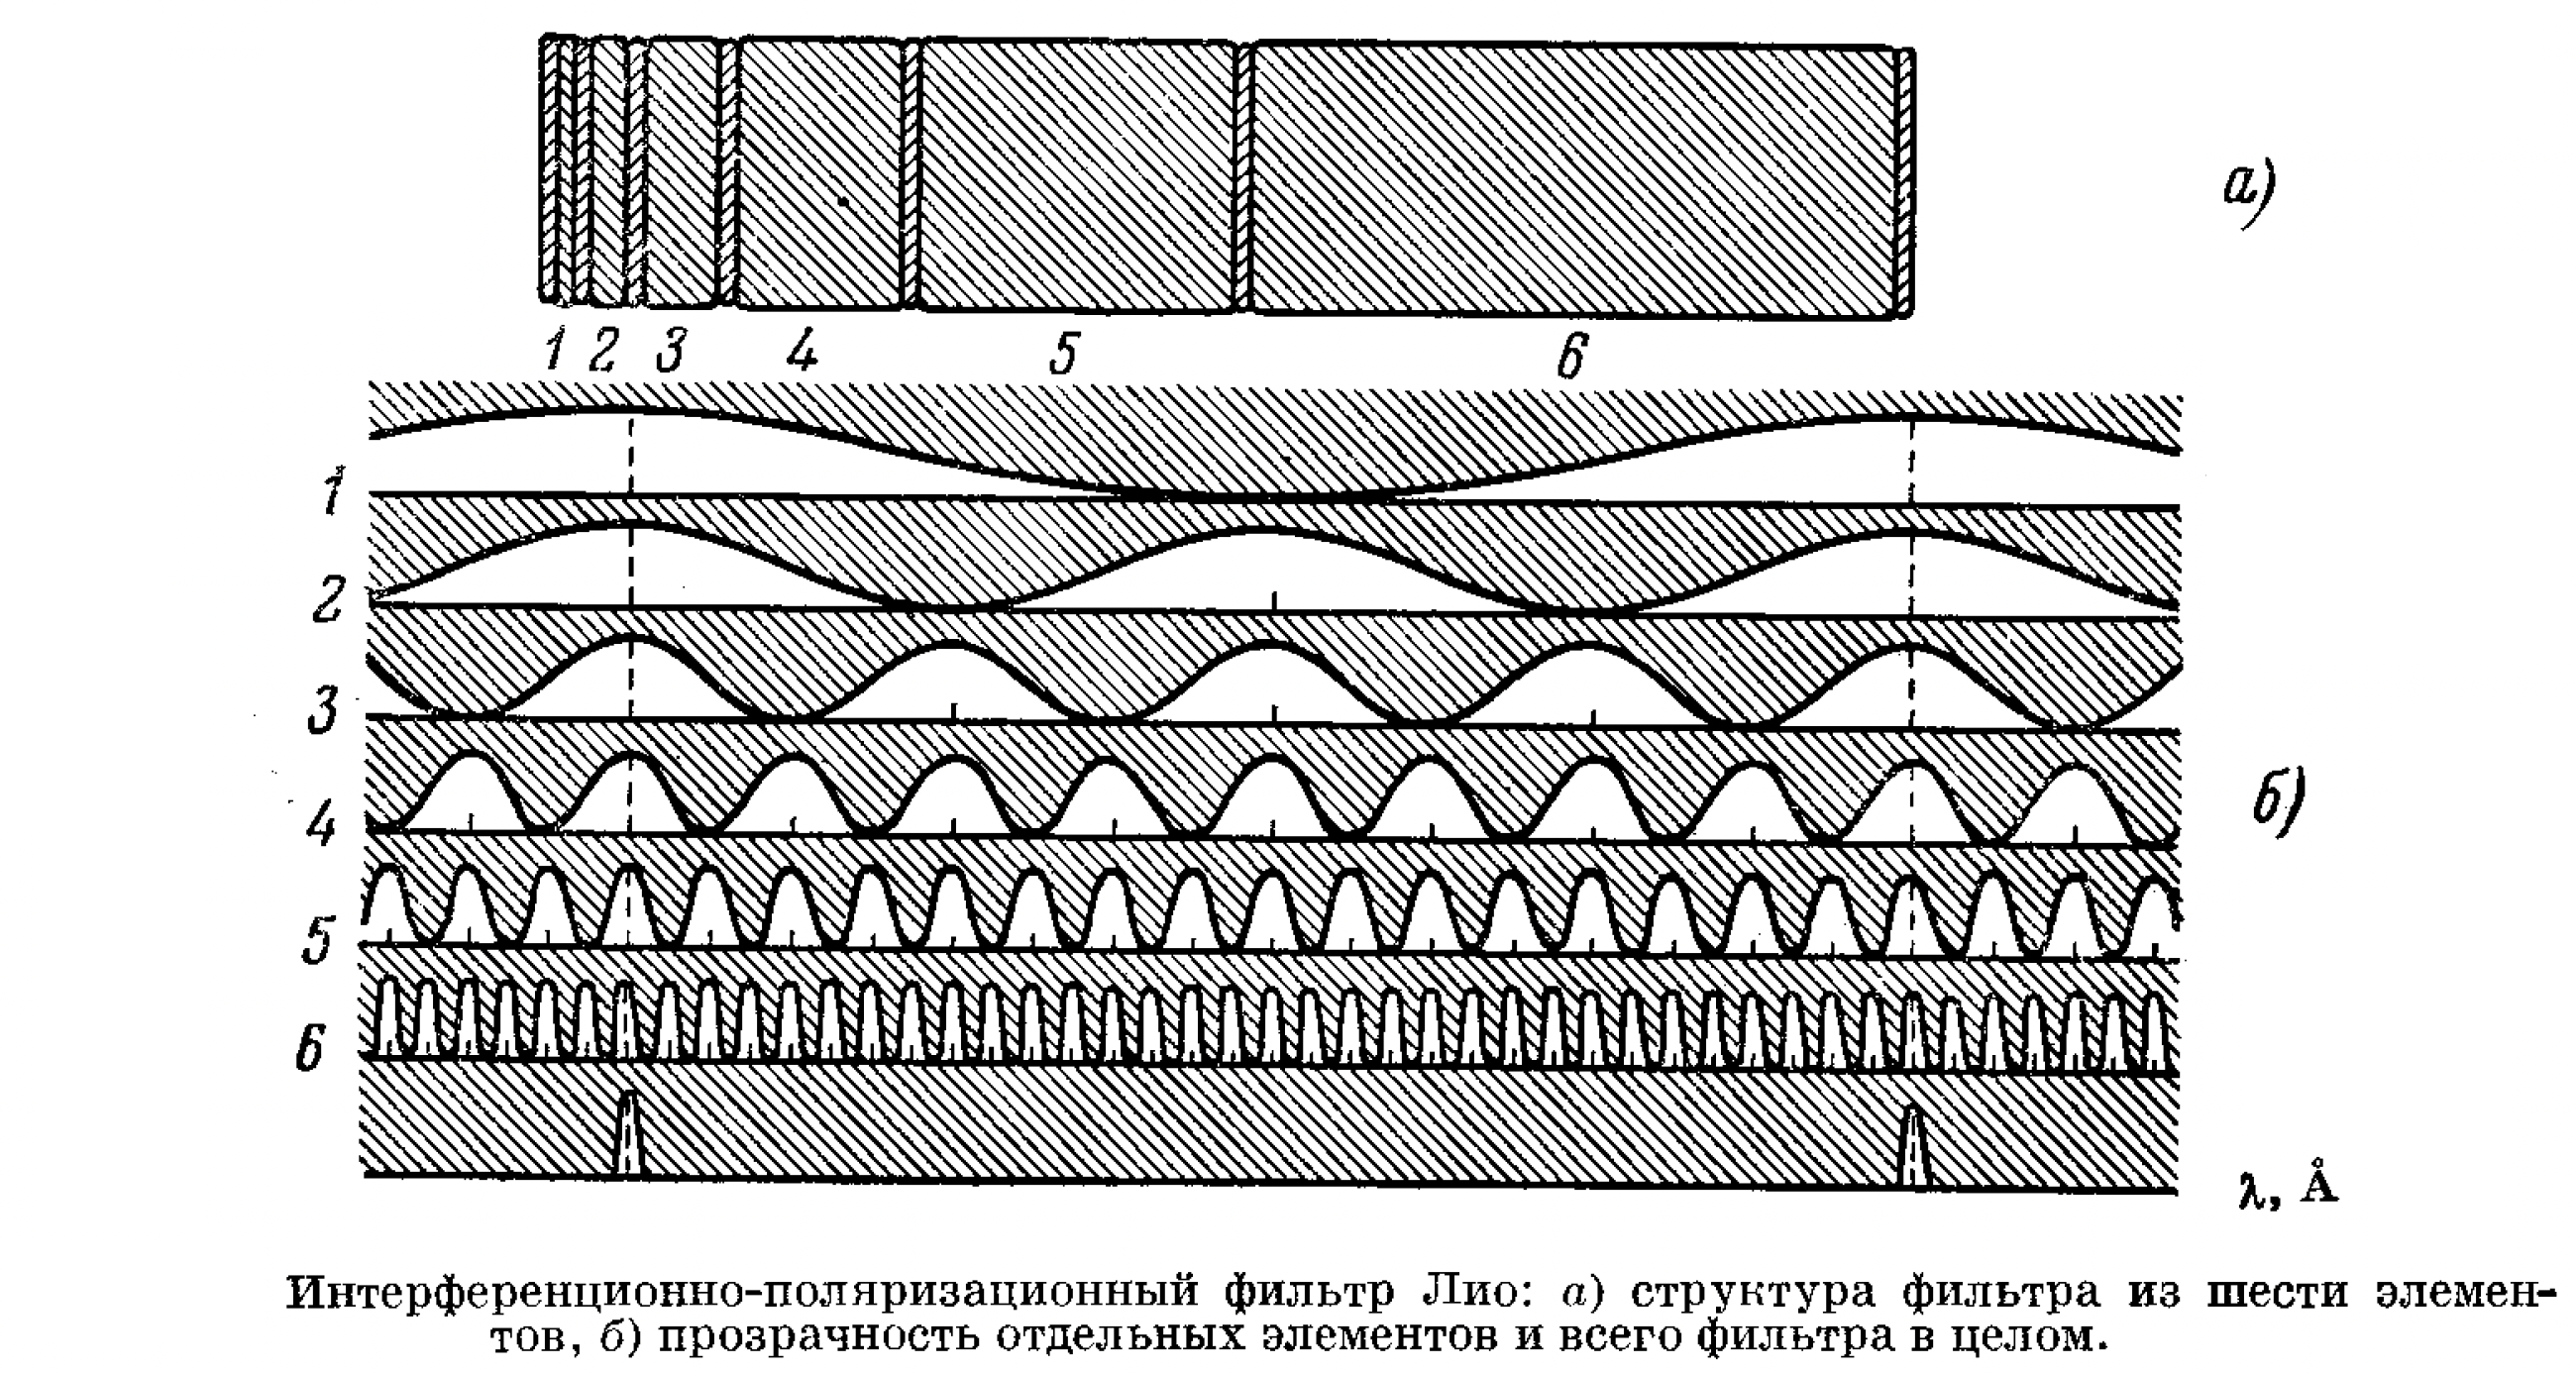
\includegraphics[scale=0.175]{03.png}    
\end{center}

\end{frame}

%7 — Свойства фильтра Лио
\begin{frame}
\frametitle{\textcolor{white}{Свойства фильтра Лио}}
Ширина полосы пропускания определяется толщиной самой толстой пластинки:
\begin{equation*}
    \Delta \lambda = \frac{\lambda^2}{2 (n_e - n_0) d}
\end{equation*}

Расстояние между полосами пропускания определяется толщиной $l$ самой тонкой пластинки.

Пропускание фильтра Лио можно вычислить как произведение соответствующих фильтров Вуда:
\begin{align*}
    T &= \cos^2 \left( \pi \frac{(n_e - n_0)d}{\lambda} \right) \cos^2 \left( 2 \pi \frac{(n_e - n_0)d}{\lambda} \right) \ldots \cos^2 \left( 2^{n - 1} \pi \frac{(n_e - n_0)d}{\lambda} \right) = \\
    &=\prod_{k = 1}^{n} \cos^2 \left( 2^{k - 1} \pi \frac{(n_e - n_0)d}{\lambda} \right) = \frac{1}{2^{2N}} \left(\frac{\sin \left( 2^N  \pi \frac{(n_e - n_0)d}{\lambda} \right)}{\sin \left(\pi \frac{(n_e - n_0)d}{\lambda} \right)}\right)^2
\end{align*}
\end{frame}

%8 — Изменение длины волны 
\begin{frame}
\frametitle{\textcolor{white}{Изменение длины волны}}
\begin{figure}[h]
\begin{minipage}[h]{0.49\linewidth}
Элементы фильтра делаются составными из двух клиньев, при смещении
одного из них толщина пластинки плавно меняется. Наклоны клиньев разных элементов и их толщины должны меняться в соответствии с геометрической прогрессией с показателем 2. Движения клиньев должны быть строго синхронизированы — рассогласование клиньев ведёт к появлению сильного фона, уменьшению пропускания в максимуме и уширению полосы пропускания.
\end{minipage}
\begin{minipage}[h]{0.49\linewidth}
\center{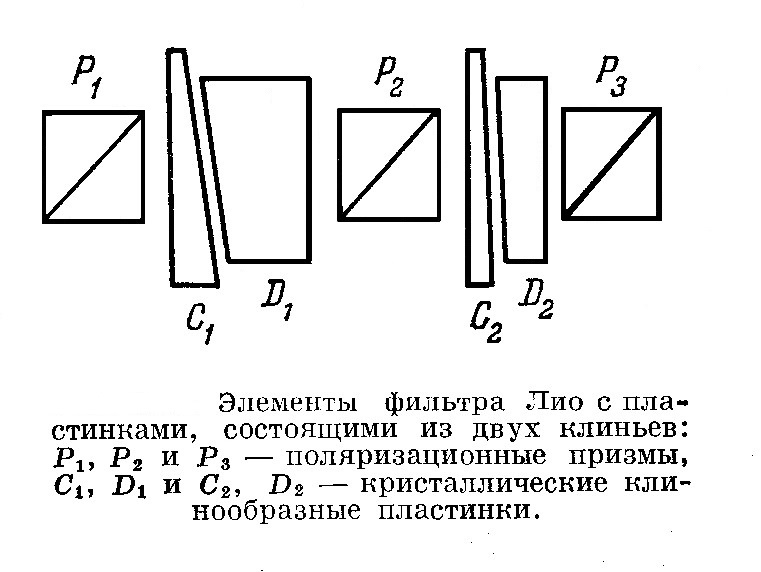
\includegraphics[scale = 0.45]{04.jpg}}
\end{minipage}
\end{figure}


\end{frame}

\begin{frame}
\frametitle{\textcolor{white}{Применение }}


Фильтр Лио позволяет получать очень узкие полосы пропускания и монохроматически фотографировать объекты с угловыми размерами от долей градуса до нескольких градусов — это находит своё применение в астрофизике.

В других конструкция плавно меняется двойное лучепреломление: этого можно достигнуть, изготовляя пластинки или их части из электрооптических кристаллов, способных менять коэффициент двойного лучепреломления под действием внешнего электрического поля
\end{frame}
\end{document}